\chapter{Introduction}
\label{ch:intro}

\section{Background and Significance}

Cardiovascular disease remains the leading cause of death worldwide, with hypertension as its primary modifiable risk factor \citep{allen2007}. Traditional cuff-based BP measurement, while clinically accurate, provides only intermittent snapshots \citep{bhs1993}. Wearable devices equipped with photoplethysmography (PPG) sensors --- the optical technique already used in smartwatches for heart-rate monitoring --- offer the possibility of continuous, cuffless BP estimation \citep{allen2007}.

\begin{figure}[htbp]
\centering
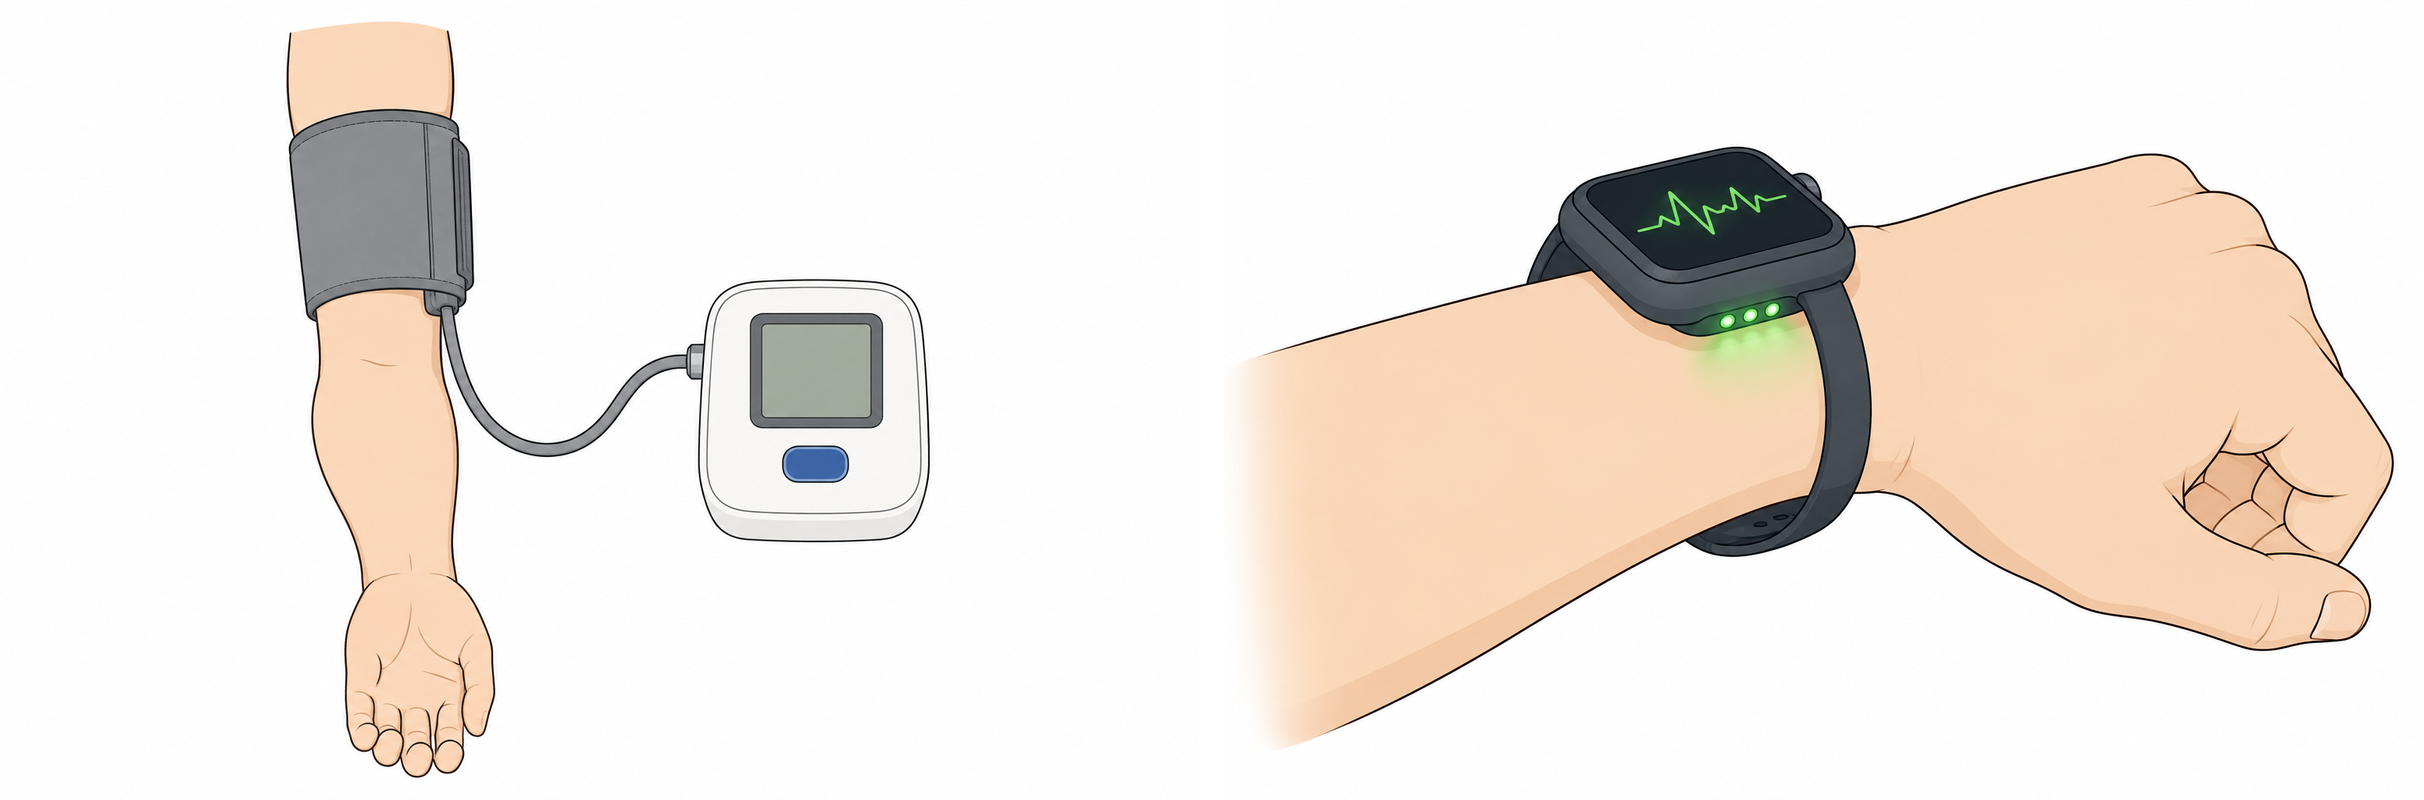
\includegraphics[width=0.85\textwidth]{figures/fig_cuff_vs_watch.png}
\caption{Conventional cuff sphygmomanometry (left) gives intermittent readings, whereas a smartwatch photoplethysmogram (right) enables continuous, cuffless monitoring.}
\label{fig:cuff_vs_watch}
\end{figure}

Despite more than a decade of research, cuffless BP estimation has yet to achieve clinical adoption \citep{mukkamala2015}. The fundamental obstacle, as this thesis demonstrates, is not signal quality or feature engineering, but cross-subject generalisation: the relationship between PPG morphology and BP varies substantially across individuals \citep{kachuee2017}.

\section{Related Work}

Cuffless BP estimation approaches fall into two broad categories. Physiology-driven methods based on pulse transit time (PTT) exploit the relationship between pulse wave velocity and arterial stiffness, but require multiple sensors and frequent individual calibration \citep{mukkamala2015}. In these methods, calibration typically fits the parameters of a physical model (for example, the coefficients of a linear PTT--BP relation) from a small number of cuff measurements, after which BP is inferred from PTT alone. Data-driven methods using machine learning learn feature-to-BP mappings from large datasets, but consistently degrade under cross-subject evaluation \citep{kachuee2017,deepppg2019}. Smartphone-based approaches have also been explored \citep{chandrasekhar2018}.

Recently, large language models have begun to be applied to physiological signal modelling. LLMs are pre-trained on vast corpora and exhibit in-context learning: they adapt to a task from a few examples without any parameter update \citep{brown2020}. For BP estimation, the motivation is twofold. First, an LLM can act as a personalised estimator that adapts to an individual through in-context calibration, avoiding the need to train a subject-specific model. Second, because LLMs are language models, physiological features can be presented not only as raw numbers but also as clinical language, allowing cardiovascular domain knowledge to be injected explicitly into the prompt. Existing work supports this direction: LLMs have been applied directly to cuffless BP measurement from wearable biosignals \citep{llmbp2024}, to health prediction from wearable sensor data \citep{healthllm2024}, and to few-shot grounding of physiological time series \citep{fewshothealth2023}. SensorLM learns sensor--language alignment through hierarchical captions \citep{sensorlm2025}, and TimeSRL proposes a semantic bottleneck to improve cross-population generalisation \citep{timesrl2026}.

The few-shot calibration proposed in this thesis differs from PTT-based calibration in three respects. First, PTT calibration fits the parameters of a fixed physical model, whereas the LLM learns the individual mapping flexibly from examples without assuming any functional form. Second, PTT requires two synchronised signals (ECG and PPG), whereas the proposed method uses PPG alone. Third, and most importantly, the LLM allows features to be expressed in clinical language, so cardiovascular domain knowledge can be injected explicitly; this is impossible in a purely numerical calibration. This thesis draws on the above work and applies LLMs to personalised BP estimation from PPG.

\section{Main Contributions}

\begin{enumerate}
  \item A few-shot personalised calibration method for cuffless BP estimation. With K chronological calibration samples, an LLM adapts to the individual at inference time, without any fine-tuning.
  \item An empirical boundary for semantic abstraction. Semantic description (retaining quantitative anchors) combined with few-shot calibration achieves SBP 5.52 / DBP 2.93 mmHg (DBP meets BHS Grade A, SBP meets Grade B), while purely qualitative summaries collapse.
  \item The finding that the LLM provides value without fine-tuning, and that semantic abstraction helps most when calibration data is scarce.
\end{enumerate}

\section{Thesis Structure}

Chapter 2 reviews technical background. Chapter 3 describes the PulseDB dataset and signal processing. Chapter 4 presents feature engineering. Chapter 5 establishes traditional ML baselines. Chapter 6 proposes the LLM few-shot calibration method. Chapter 7 investigates semantic abstraction. Chapter 8 concludes.
